\documentclass[10pt,conference]{IEEEtran} 
\IEEEoverridecommandlockouts
% The preceding line is only needed to identify funding in the first footnote. If that is unneeded, please comment it out.
\usepackage{cite}
\usepackage{amsmath,amssymb,amsfonts}
\usepackage{algorithmic}
\usepackage{graphicx}
\usepackage{textcomp}
\usepackage{booktabs}
\usepackage[table,xcdraw]{xcolor}
\usepackage{xcolor}
\definecolor{mypink3}{cmyk}{0, 0.7808, 0.4429, 0.1412}

\def\BibTeX{{\rm B\kern-.05em{\sc i\kern-.025em b}\kern-.08em
    T\kern-.1667em\lower.7ex\hbox{E}\kern-.125emX}}
	
\begin{document}

\title{Security vs. Maintainability: Fixing Vulnerabilities Obfuscates your Code\\
\thanks{Identify applicable funding agency here. If none, delete this.}
}

\author{
    Anonymou(s) Author(s)
%     \IEEEauthorblockN{1\textsuperscript{st} Given Name Surname}
% \IEEEauthorblockA{\textit{dept. name of organization (of Aff.)} \\
% \textit{name of organization (of Aff.)}\\
% City, Country \\
% email address}
% \and
% \IEEEauthorblockN{2\textsuperscript{nd} Given Name Surname}
% \IEEEauthorblockA{\textit{dept. name of organization (of Aff.)} \\
% \textit{name of organization (of Aff.)}\\
% City, Country \\
% email address}
% \and
% \IEEEauthorblockN{3\textsuperscript{rd} Given Name Surname}
% \IEEEauthorblockA{\textit{dept. name of organization (of Aff.)} \\
% \textit{name of organization (of Aff.)}\\
% City, Country \\
% email address}
}

\maketitle

\begin{abstract}

Lorem Ipsum is simply dummy text of the printing and typesetting industry. 
Lorem Ipsum has been the industry's standard dummy text ever since the 1500s, 
when an unknown printer took a galley of type and scrambled it to make a type 
specimen book. It has survived not only five centuries, but also the leap into 
electronic typesetting, remaining essentially unchanged. It was popularised in 
the 1960s with the release of Letraset sheets containing Lorem Ipsum passages, 
and more recently with desktop publishing software like Aldus PageMaker including 
versions of Lorem Ipsum. It was popularised in the 1960s with the release of 
Letraset sheets containing Lorem Ipsum passages, and more recently with desktop 
publishing software like Aldus PageMaker including versions of Lorem Ipsum.

\end{abstract}

\begin{IEEEkeywords}
Security, Maintainability, Open-Source
\end{IEEEkeywords}

\section{Introduction}



Add a point for motivation with one of the examples of the poster.

\section{Related Work}



\section{Methodology}



\subsection{Dataset}

\begin{table*}[h]
\centering
\caption{Descriptive statistics of the dataset projects\textcolor{mypink3}{@update}} \label{tab:dataset} 
\begin{tabular}{@{}ccccccccccc@{}}
\toprule
     & forks   & stars   & watchers & contributors & commits  & branches & releases & size      & issues  & pull requests \\ \midrule
Mean & 1734.79 & 5262.97 & 395.11   & 152.48       & 22257.82 & 44.08    & 126.31   & 143243.64 & 3725.4  & 1976.92       \\
Min     & 1       & 3       & 1        & 0            & 103      & 1        & 0        & 108       & 0       & 0             \\
25 \%     & 374.75  & 1571.5  & 117.75   & 48           & 1347     & 4        & 22       & 8339.5    & 321.25  & 151.75        \\
Median     & 887     & 2836.5  & 258.5    & 102.5        & 5823     & 9        & 59       & 38331.5   & 1652.5  & 515.5         \\
75 \%     & 2196    & 6455.75 & 462.5    & 259          & 22786.25 & 22.25    & 142.25   & 164442.5  & 4152.75 & 1944.25       \\
Max     & 16366   & 31841   & 3446     & 413          & 717449   & 1227     & 1114     & 2042017   & 33970   & 19329         \\
Total     & 180418  & 547349  & 41091    & 15858        & 2314813  & 4584     & 13136    & 14897339  & 387442  & 205600        \\ \bottomrule
\end{tabular}
\end{table*}



\subsection{Security vs. Baseline Commits}



\subsection{Maintainability}


\begin{figure}[h]
 	\centering
 	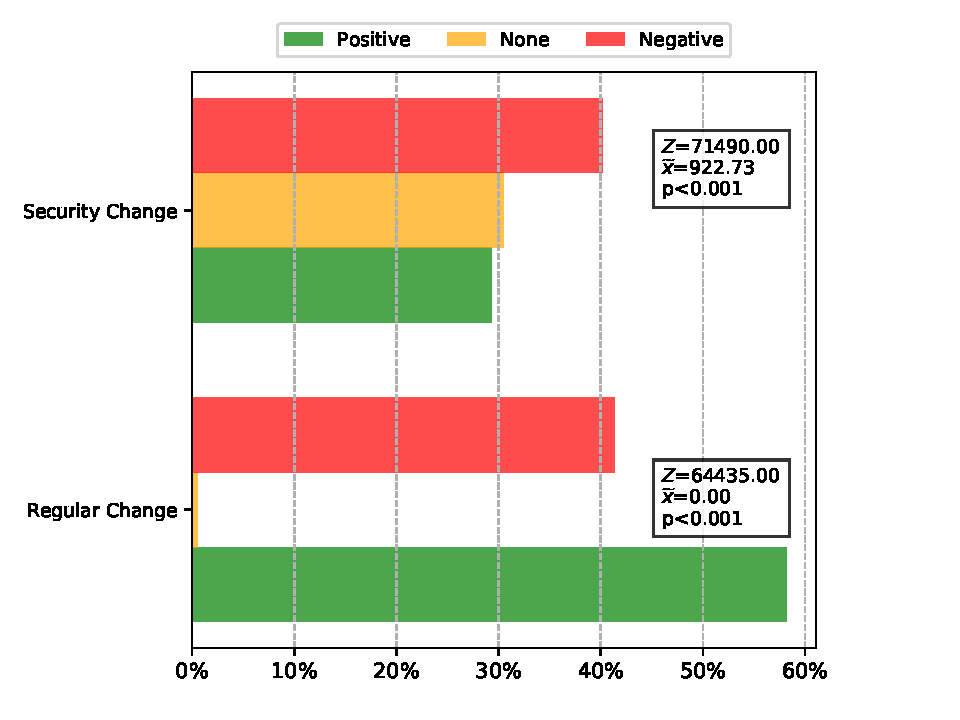
\includegraphics[width=0.5\textwidth]{figures/maintainability.pdf}
 	\caption{Maintainability difference for security and baseline commits \textcolor{mypink3}{@update}}
\end{figure}


\cite{Wang:2008:DSJ:1330017.1330021}


\section{Results}




\section{Discussion}


\section{Threats to Validity}


\section{Conclusion}



\section*{Acknowledgment}

{
 \bibliographystyle{IEEEtran}
  \bibliography{icpc19}
}

\end{document}
